The user selects the artist's biography (for completeness) and birth (for validation). Karma then automatically constructs SPARQL queries for the data.
To facilitate the integration for this demo, we generated owl:sameAs links between the datasets' artists using LIMES \cite{ngomo2011limes}.  In future work we will investigate adding this process for the user.
Karma then merges the results and updates the source model appropriately as illustrated in Figure~\ref{fig:augment-screenshot}, so the user can continue to explore the integrated data interactively. 

\begin{figure*}
\begin{center}
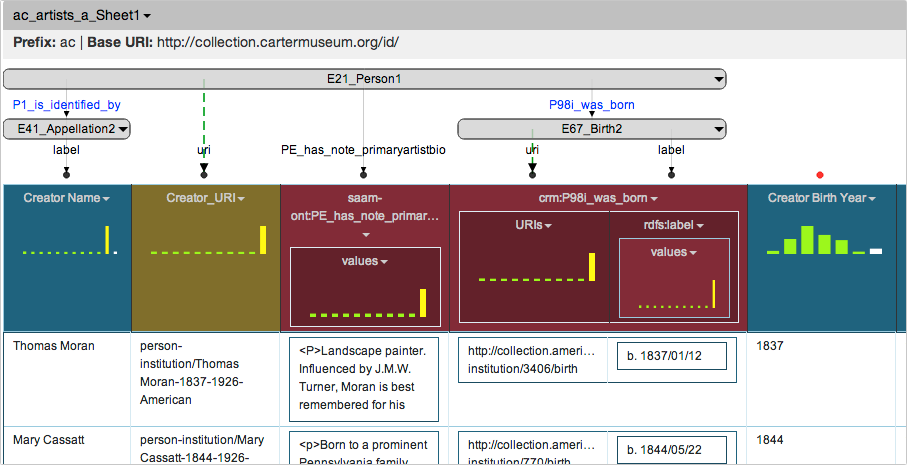
\includegraphics[width=4.9in]{images/6-augment.png}
\vspace{-3mm}
\caption{A Karma user has integrated biographical data from the Smithsonian into their dataset}
\vspace{-2mm}
\label{fig:augment-screenshot}
\end{center}
\vspace{-1.5em}
\end{figure*}
